\documentclass{article}
\usepackage[utf8]{lipsum}
\usepackage{color}
\usepackage{graphicx}
\title{\textbf{CSE300 Assignment1 \\
Introduction to \LaTeX}\\ \textbf{\hugeTarget Enumeration via Euler Characteristic
Integrals
}}
\author{ Madhusudan Basak \\
Mahmudur Rahman Hera \\
Student ID: 1505071 }

\begin{document}
\maketitle
\vspace{1.5in}

\begin{figure}[h]
    \centering
    
\includegraphics[width=100]{graphics/buetlogo.png}
\end{figure}
\centering Department of Computer Science and Engineering \\
\centering Bangladesh University of Engineering and Technology \\
\centering (BUET) \\
\centering Dhaka 1000 \\
\centering \date{\today}
\newpage
\tableofcontents
\newpage

\textbf{Abstract} \\
\begin{flushleft}

\normalsize {We solve the problem of counting the total number of observable targets (e.g., persons, vehicles, landmarks) in a region using local counts performed by a network of sensors, each of which measures the number of targets nearby but neither their identities nor any positional information. We formulate and solve several such problems based on the types of sensors and mobility of the targets. The main contribution of this paper is the adaptation of a topological sheaf integration theory integration with respect to Euler characteristic — to yield complete solutions to these problems.}
\\
\textbf{Key words:} Euler characteristic, sensor network, enumeration, integration

\section{Topological enumeration.}
\subsection{Sensors.}

Sensor networks are poised to impact society in fundamental ways analogous to the impact of the personal computer and the internet. The rapid development of small-scale sensor devices coupled with wireless ad hoc networking capability
is giving birth to a wide variety of sensor networks for applications to agriculture, defense, environmental monitoring, and more.
\\

\subsection{A simple example: Geometric enumeration.}
The following simple example of target enumeration has a trivial geometric solution that motivates our topological techniques. Consider a field of (infinitesimally small) sensors, one at each point x in a planar domain  ${\rm I\!R}$. Assume there is a finite set of points acting as observables or targets  O_\alpha \subset  ${\rm I\!R}$, and that the sensor at x \in   ${\rm I\!R}$ returns a quantized count h(x)\in N ~.
\\
\hspace{5mm} How can sensors merge their local counts into a global count of the number of targets? If the targets are sufficiently separated, then this becomes a simple problem of counting the number of connected “on” clusters in the network . If we want
to allow for more complex target interactions, the following critical (if not entirely
realistic) assumption makes the problem very simple.Then the total number of targets may be computed as an integral:

\end{flushleft}

\begin{equation}

   O_\alpha=\frac{1}{M} \int_{\textbf{R}^2} h(x) dx \hspace{1in}
   \label{eqn:e}
\end{equation}
\\
\begin{flushleft}
Where\[M =\pi {\textbf{R}}^2 \]
\[h = \sum_\alpha \textbf{l} U_\alpha\]
\end{flushleft}

\begin{figure}[h]
    \centering
    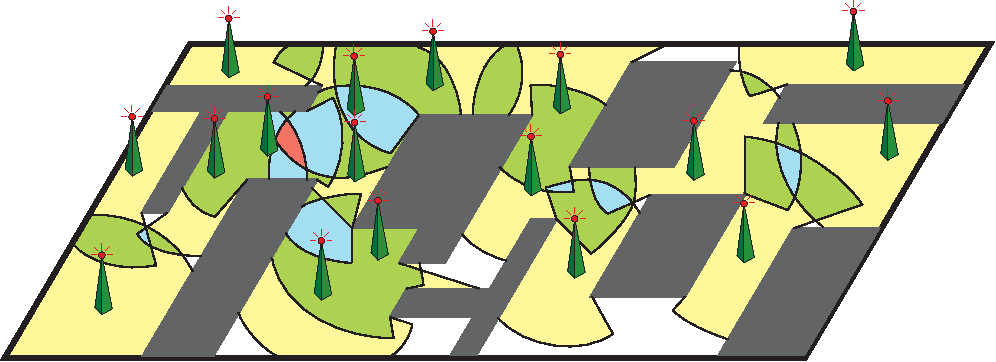
\includegraphics[width=300]{graphics/fig2.png}
\end{figure}
\centering{Fig.1 . A sensor field counts the number of in-range visible beacons based on line-of-sight. Target supports (the region in the sensor space from which the target is sensed) may vary greatly in size and shape, depending on beacon strength and target space obstacles; however, target supports are star-convex with respect to the target and thus all topologically trivial.}

\begin{flushleft}
\subsection{Other problem statements.}
There are numerous interesting and challenging problems that involve determining a global count based on a local count. Some variants we address in this paper include the followin

\begin{enumerate}
    \item  Each sensor sweeps a finite length beam or cone over all bearings, recording the number of targets sensed as a function of bearing and locatio
    \item Each sensor increments an internal counter whenever a moving target comes
within rang.
\item  Each sensor increments an internal counter whenever a moving wave front.
initiated by a target event passes within rang
\end{enumerate}

\section{Integration with respect to Euler characteristic.}
Our results follow from the classical and elegant theory of integration with respect to Euler characteristic. We restrict attention to subsets of \textbf{R}^2.
\subsection{The simplicial approach.}
For simplicity, we begin our treatment of topological
integration with simplicial complexes (triangulated piecewise-linear sets) in Rn.
For $\kappa \geq 0 $, a  $\kappa-simplex,\sigma$, is the convex hull of a set of $\kappa + 1$  affinely  independent  vertices   {V_i}_0^k ~ in \\
\[\textbf{R^n}:\sigma=\{\sum_i t_iv_i :t_i \in (0,1),\sum_i t_i=1 \} \].
\end{flushleft}
\\
The geometric Euler characteristic of a simplicial complex X is \\
\begin{equation}

\[${}_{\chi}\chi=\sum_\sigma (-1)^{dim
\sigma}=\sum_\kappa^\infty (-1)^\kappa \hspace{2in} $\]
\end{equation}
\begin{flushleft}
Here $\kappa $ simplices  in  \chi .
\end{flushleft}
\vspace{1in}

\begin{wrapfigure}{L}{0.45\textwidth}
    \centering
    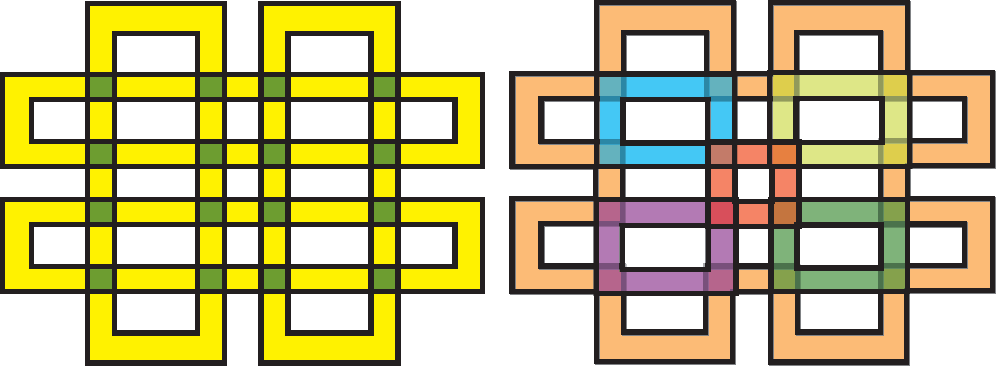
\includegraphics[scale=.4]{graphics/fig3.png}
\end{wrapfigure}
fig.2 .$h = \sum_\alpha \textbf{l} U_\alpha$ ~ with ${}_{\chi}(U_\alpha)=0\]$,one has $\sum h dx=0$ .
 It is not possible in general
to determine $#\alpha$. (Left) The height function of a collection of annuli. Four? or (right) six? Any
even number between two and twelve is possible with embedded annuli
\begin{flushleft}
\subsection{The definable approah.}
 
We extend the definitions to a wide class of spaces which are not obviously simplicial. The reader who is in a hurry may skip ahead to section 3 and remain in the class of simplicial complexes. Not all sets are measurable in $d\chi$: Cantor sets, Hawaiian  earrings, and  other “wild” sets do not  possess  a  well-defined  Euler  characteristic. 

\subsection{The sheaf approach.}
. There is, as intimated earlier, a deeper treatment
in the literature on sheaves. There are significant and deep perspectives from sheaf
theory that can be easily interpreted in the setting of Euler integration.
A sheaf is, roughly speaking, a means of assigning to open sets of a topological
space some algebraic object (e.g., a group) in a manner that respects the operations of
(1) restriction and (2) gluing. The canonical example of a sheaf on a space X is C(X),
the continuous functions X \rightarrow R.

\begin{figure}[h]
    \centering
    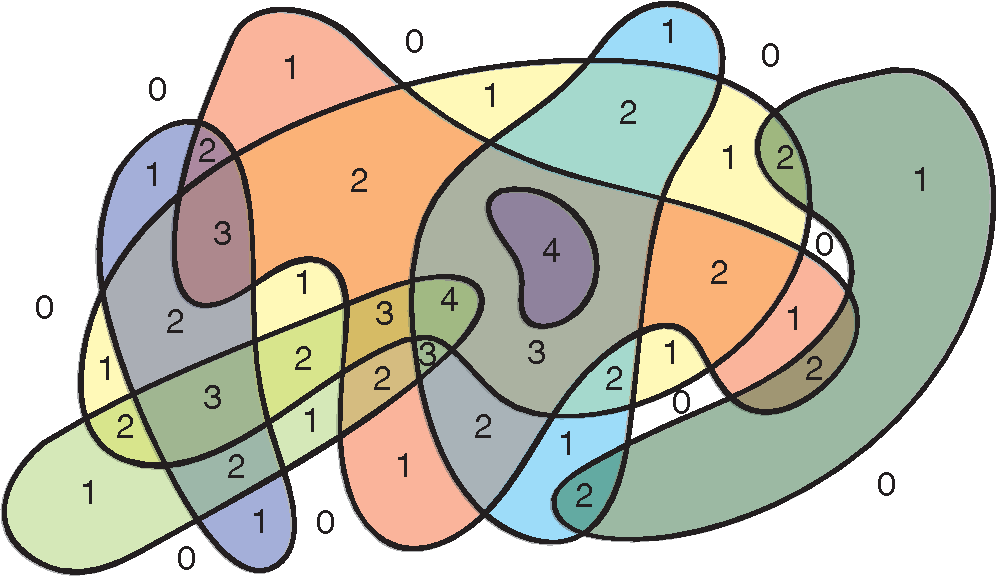
\includegraphics[width=300]{graphics/fig4.png}
\end{figure}
\\
Fig.3 .A collection of contractible patches $U_\alpha$ in  $\textbf{R^2}$ corresponding to the supports or “visibility regions” of seven targets.
\end{flushleft}
\\
\begin{flushleft}

\section{From fields to networks.}
\\
The mathematical tools formulated here for enumeration
problems depend on having a sensor field with counting data at all points
in a continuum of the sensor space. Any realistic implementation must occur over a
discrete collection of sensors: a network, where nodes N (typically within the target
space N \subset W) record values.
\\
~~~ Trying to parameterize the sensor space X as a discrete set based on the nodes N
is doomed to failure, as the target supports will be likewise discrete and of unknown
and nonuniform Euler characteristic. Likewise, if the communication links between
nodes give the sensor network the structure of a graph, then the network graph is an
equally bad candidate for the sensor space X: cycles in the graph can make the Euler
characteristics of the target supports vary greatly. In fact, the denser the network in
W, the more negative the Euler characteristics of the target supports become (e.g.,
in Figures 5, 6, and 7, the target supports intersected with the network are graphs
with negative Euler characteristic).
\subsection{Numerical analysis and Euler integrals.}
A more sensible parametrization
is to model the sensor space X as a simplicial approximation to the target space
W, using the nodes N as vertices. Assume that enough structure is known about
N to give a simplicial structure (a triangulation) that has N as the vertex set. In
analogy with the problem of computing a numerically approximate Riemann integral
of an integrand h based on a discrete sampling, one guesses that the integral of the
piecewise-linear (PL) interpolation $h_{PL}$ of h based on the sampled values at N is a
good approximation.
\end{flushleft}
\vspace{.5in}

\begin{figure}[h]
    \centering
    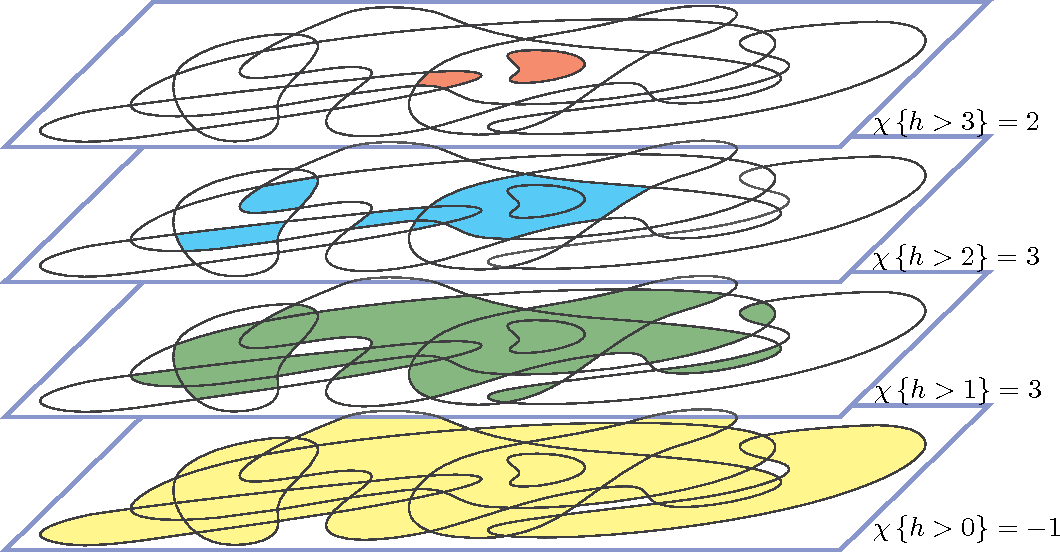
\includegraphics[width=300]{graphics/fig5.png}
\end{figure}
\\
Fig.4 Decomposing h into upper excursion sets and computing χ yields the integral $\int h d\kappa.$
\begin{flushleft}
\subsection{Ad hoc planar networks.}
We note that the strategy of converting the
sampling of the true impact function h over N to a PL interpolation $h_{PL}$ does not
necessarily require knowing the coordinates of the nodes. Indeed, the evaluation of
$$\int_\kappa d\kappa $ is conspicuous in its freedom from coordinate geometry: it is a topological
integral. If one is given a triangulation, the extension of the counting function h
on vertices over the domain is automatic. However, if no geometry associated with
N is known, it may not be possible to determine a canonical extension $h_{PL}$ over
the domain. Such a situation is not uncommon in sensor networks based on ad
hoc wireless communications, an increasingly common protocol for distributed sensor
networks and robotics.
\end{flushleft}

\end{document}